% begin module hyperbolic-functions-def
% % % % % % % % % % % % % % % % % % % % % %
\begin{frame}
The hyperbolic functions satisfy a number of identities that are similar to well-known trigonometric identities.\\
We list some of them here and leave most of the proofs as (easy?) exercises.

\begin{definition}[(some) Hyperbolic Identities]
\[
\begin{array}{l@{\extracolsep{2cm}}l}
\sinh(-x) = -\sinh x & \cosh (-x)=\cosh x\\ [3mm]

\cosh^2(x)-\sinh^x x = 1   & 1-\tanh^2 x = \sech^2 x\\ [3mm]
\end{array}
\]
\[
\sinh(x+y)=\sinh x\cosh y+\cosh x \sinh y
\]
\[
\cosh(x+y)=\cosh x\cosh y+\sinh x \sinh y
\]
\end{definition}




\end{frame}
% % % % % % % % % % % % % % % %
\begin{frame} 
\begin{example}
Prove $\cosh^2x - \sinh^2x = 1$ and $1 - \tanh^2x = \sech^2x$.\\
\textbf{Solution:\\} \pause 
\begin{align*}
\cosh^2x - \sinh^2x & = \left(\frac{e^x+e^{-x}}{2}\right)^2 - \left(\frac{e^x-e^{-x}}{2}\right)^2\\
\onslide<3->{&= \frac{e^2x+2+e^{-2x}}{4}- \frac{e^2x-2+e^{-2x}}{4}}\\
\onslide<4->{& = \frac44 = 1}
\end{align*}
\onslide<5->{For the second identity we use the first to get}
\onslide<6->{
\begin{align*}
\cosh^2x - \sinh^2x = 1 & \;\To\; \frac{\cosh^2x}{\cosh^2x}-\frac{\sinh^2x}{\cosh^2x}= \frac{1}{\cosh^2x}\\
\onslide<7->{&\;\To\; 1 -\tanh^2x = \sech^2x} 
\end{align*}
}

\end{example}
\end{frame}

% % % % % % % % % % % % % % % % % % % % % % % % %
\begin{frame} 
\frametitle{Why ``Hyperbolic Trig"?}

\begin{columns}
\begin{column}{.5\linewidth}
\begin{figure}
\centering
\psset{xunit=1cm, yunit=1cm}
\begin{pspicture}(-2.4, -2.4)(2.4,2.4)
\fcAxesStandard{-2.2}{-2.2}{2.2}{2.2}
\fcLabels{2.2}{2.2}
\pscustom*[linecolor=\fcColorAreaUnderGraph]{
\psline*(0,0)(1,0)
\parametricplot{0}{60}{t cos t sin}
\psline(! 60 cos 60 sin)(0,0)
}
\parametricplot[linecolor=\fcColorGraph]{0}{360}{t cos t sin}
\fcFullDot{60 cos }{60 sin}
\rput[l](! 60 cos 0.1 add 60 sin ){$P(\cos t, \sin t)$}
\fcFullDot{1}{0}
\rput[lt](1, -0.1){$Q$}
\parametricplot[linecolor=green]{0}{60}{t cos t sin}
\psline[linecolor=blue](0,0)(1,0)
\psline[linecolor=blue](! 60 cos 60 sin)(0,0)
\rput[tl](0.3, -1.2){$x^2+y^2=1$}
\end{pspicture}
%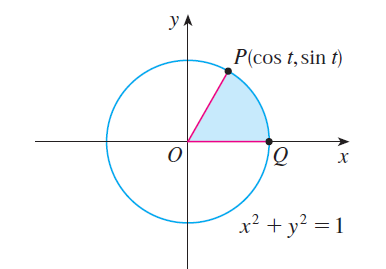
\includegraphics[width=\linewidth]{../../modules/hyperbolic-functions/pictures/trigCircle}
\caption{Trig functions are ``circular": $t$ is the measure of the angle, which (as we know) is equal to twice the area of the shaded circular sector.}
\label{fig:trigCircle}
\end{figure}

\end{column}
\begin{column}{.5\linewidth}
\pause 
\begin{figure}
\centering
\psset{xunit=1cm, yunit=1cm}
\begin{pspicture}(-2.4, -2.4)(2.4,2.4)
\fcAxesStandard{-2.2}{-2.2}{2.2}{2.2}
\fcLabels{2.2}{2.2}
\pstVerb{
/sinh {dup 2.718281828 exch exp exch -1 mul 2.718281828 exch exp sub 2 div} def
/cosh {dup 2.718281828 exch exp exch -1 mul 2.718281828 exch exp add 2 div} def
/theAngle 1.3 def
}
\pscustom*[linecolor=\fcColorAreaUnderGraph]{
\psline*(0,0)(1,0)
\parametricplot{0}{theAngle}{t cosh t sinh}
\psline(! theAngle cosh theAngle sinh)(0,0)
}
\parametricplot[linecolor=\fcColorGraph]{-1.5}{1.5}{t cosh t sinh}
\parametricplot[linecolor=\fcColorGraph]{-1.5}{1.5}{t cosh -1 mul t sinh}
\fcFullDot{theAngle cosh }{theAngle sinh}
\rput[r](! theAngle cosh 0.1 sub theAngle sinh ){$P(\cosh t, \sinh t)$}
\fcFullDot{1}{0}
\rput[lt](1, -0.1){$Q$}
\parametricplot[linecolor=green]{0}{theAngle}{t cosh t sinh}
\psline[linecolor=blue](0,0)(1,0)
\psline[linecolor=blue](! theAngle cosh theAngle sinh)(0,0)
\rput[tl](0.1, -1.4){$x^2-y^2=1$}
\end{pspicture}
%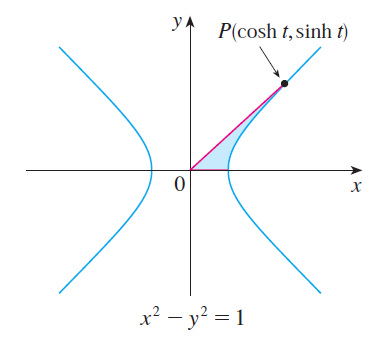
\includegraphics[width=\linewidth]{../../modules/hyperbolic-functions/pictures/hyperbolicSector}
\caption{Here $ t $ represents twice the area of the shaded hyperbolic sector..}
\label{fig:hypCircle}
\end{figure}

\end{column}
\end{columns}

\end{frame}

% end module
